\documentclass{beamer}
%% \documentclass[handout]{beamer}

% \usetheme{Antibes}
% \usetheme{Berlin}
\usetheme{CambridgeUS}
% \usetheme{Copenhagen}

\usepackage{hyperref}
\usepackage{caption}
\usepackage{ytableau}
\usepackage{tikz-cd}
\usepackage{centernot}
\usepackage[shortlabels]{enumitem}
\usepackage{cases}
\usepackage{bbm}
\usepackage{tikz}

\usepackage{ytableau}

\usetikzlibrary{arrows.meta, positioning, shapes.geometric}
\usetikzlibrary{shadows}

\newtheorem{thm}{Theorem}[section]
\newtheorem{conjecture}{Conjecture}[section]
\newtheorem{lem}[thm]{Lemma}
\newtheorem{prop}[thm]{Proposition}
\newtheorem{cor}[thm]{Corollary}
\newtheorem{conj}[thm]{Conjecture}
\theoremstyle{definition}
\newtheorem{exam}[thm]{Example}
\newtheorem{prob}[thm]{Problem}
\newtheorem{defn}[thm]{Definition}
\newtheorem{observation}{Observation}
\newtheorem{remark}[thm]{Remark}
\newtheorem*{StanleyStembridge}{Stanley--Stembridge conjecture (1993)}
\newtheorem*{OpenProblem}{Open problem}
\newtheorem*{FKnonneg}{Fomin--Kirillov nonnegativity conjecture (1999)}

\newcommand\ZZ{\mathbb{Z}}
\newcommand\NN{\mathbb{N}}
\newcommand\QQ{\mathbb{Q}}
\newcommand\RR{\mathbb{R}}
\newcommand\CC{\mathbb{C}}
\newcommand\FF{\mathbb{F}}


\newcommand\xx{\mathbf{x}}

\newcommand\KL{\operatorname{KL}}
\newcommand\TL{\operatorname{TL}}

\newcommand\remph[1]{\emph{\textcolor{red}{#1}}}
\newcommand\bemph[1]{\emph{\textcolor{blue}{#1}}}

\title[Mathematical research in AI era]{Mathematical research in AI era}
\author[Byung-Hak Hwang]{Byung-Hak Hwang}
\institute[KIAS]{KIAS CAINS}
\date[]{CAINS Welcome Talk \\ April 15 2026}

%%%%%%%%%%%%%%%%%%%%%%%%%%%%%%%%%%%%%%%%%%%%%%

\AtBeginSection[]{%
\begin{frame}
    \tableofcontents[currentsection, subsectionstyle=show/show/hide]
\end{frame}
}

%%%%%%%%%%%%%%%%%%%%%%%%%%%%%%%%%%%%%%%%%%%%%%

\begin{document}

\begin{frame}
  \titlepage
\end{frame}

%%%%%%%%%%%%%%%%%%%%%%%%%%%%%%%%%%%%%%%%%%%%%%

\begin{frame}
  \frametitle{Two approaches to AI for mathematics}
  \pause
  Research on AI for mathematics can be broadly divided into two directions:
  \vspace{.5cm}
  \pause

  \begin{itemize}
    \item[\textbf{I.}] \bemph{Data-scientific approach} \\
      Use machine learning to explore mathematical objects, detect hidden
      patterns, and guide mathematicians towards new conjectures and proofs.
      \vspace{.3cm}
      \pause
    \item[\textbf{II.}] \bemph{Interactive \& automated theorem proving} \\
      Use proof assistants (Lean, Coq, Isabelle) and learning-based agents
      to formalize, verify, and eventually generate mathematical proofs.
  \end{itemize}
\end{frame}

%%%%%%%%%%%%%%%%%%%%%%%%%%%%%%%%%%%%%%%%%%%%%%

\section{Data-scientific approach}

%%%%%%%%%%%%%%%%%%%%%%%%%%%%%%%%%%%%%%%%%%%%%%

\begin{frame}
  \frametitle{A framework for AI-guided mathematical discovery}
  \begin{center}
    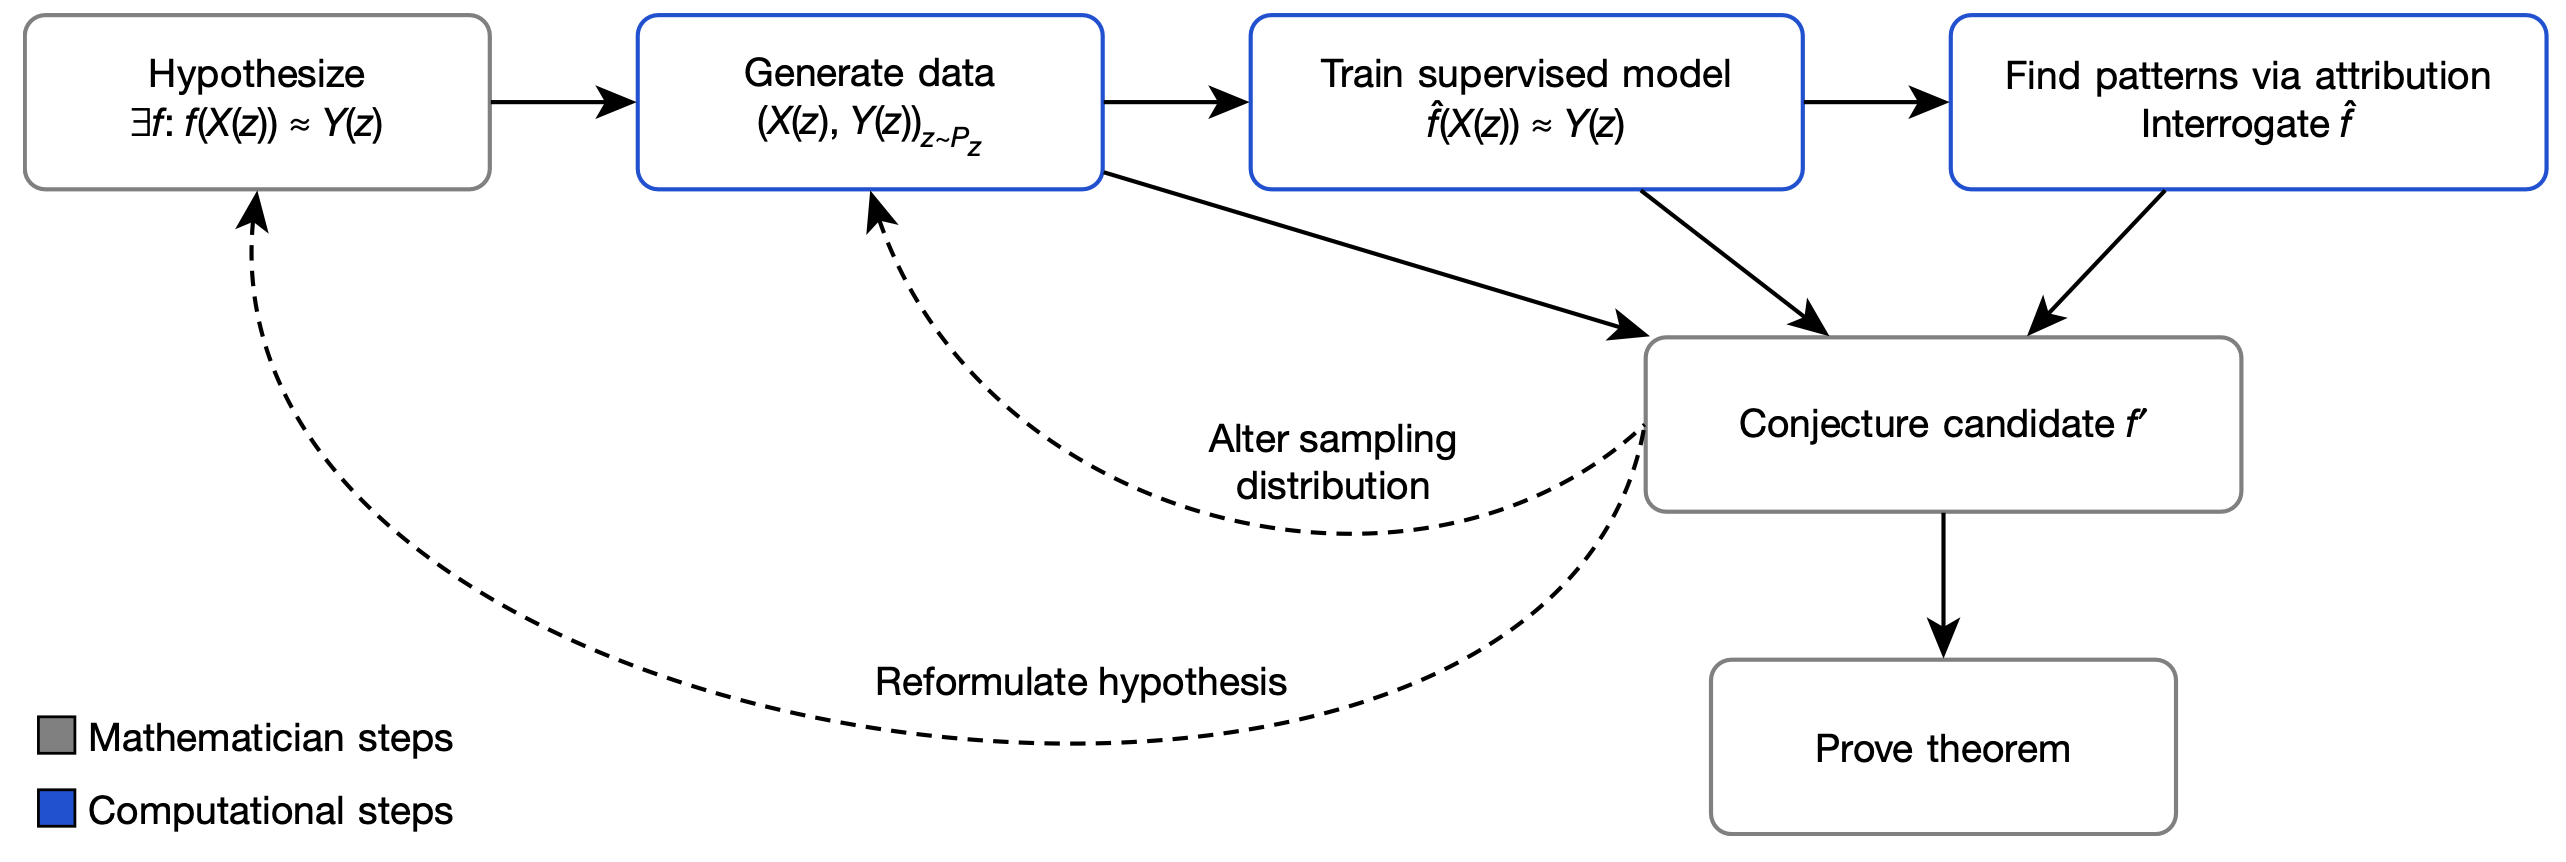
\includegraphics[width=\textwidth]{./figures/AI-driven-research-diagram.png}
  \end{center}
  \begin{flushright}
    \small Davies et al., \emph{Nature} (2021)
  \end{flushright}
\end{frame}

%%%%%%%%%%%%%%%%%%%%%%%%%%%%%%%%%%%%%%%%%%%%%%

\begin{frame}
  \frametitle{Case 1: Kazhdan--Lusztig polynomials and the hypercube decomposition}
  For a Coxeter group \( W \), each pair \( u \le v \) of elements in Bruhat order
  carries a \emph{Kazhdan--Lusztig polynomial} \( P_{u,v}(q) \in \ZZ[q] \), fundamental
  in representation theory and geometry of Schubert varieties.
  \vspace{.2cm}
  \pause

  \begin{conjecture}[Combinatorial Invariance, Lusztig--Dyer, 1980s]
    \( P_{u,v}(q) \) depends only on the Bruhat interval \( [u,v] \) as a poset.
  \end{conjecture}
  \pause

  \only<1-3>{
  \begin{center}
    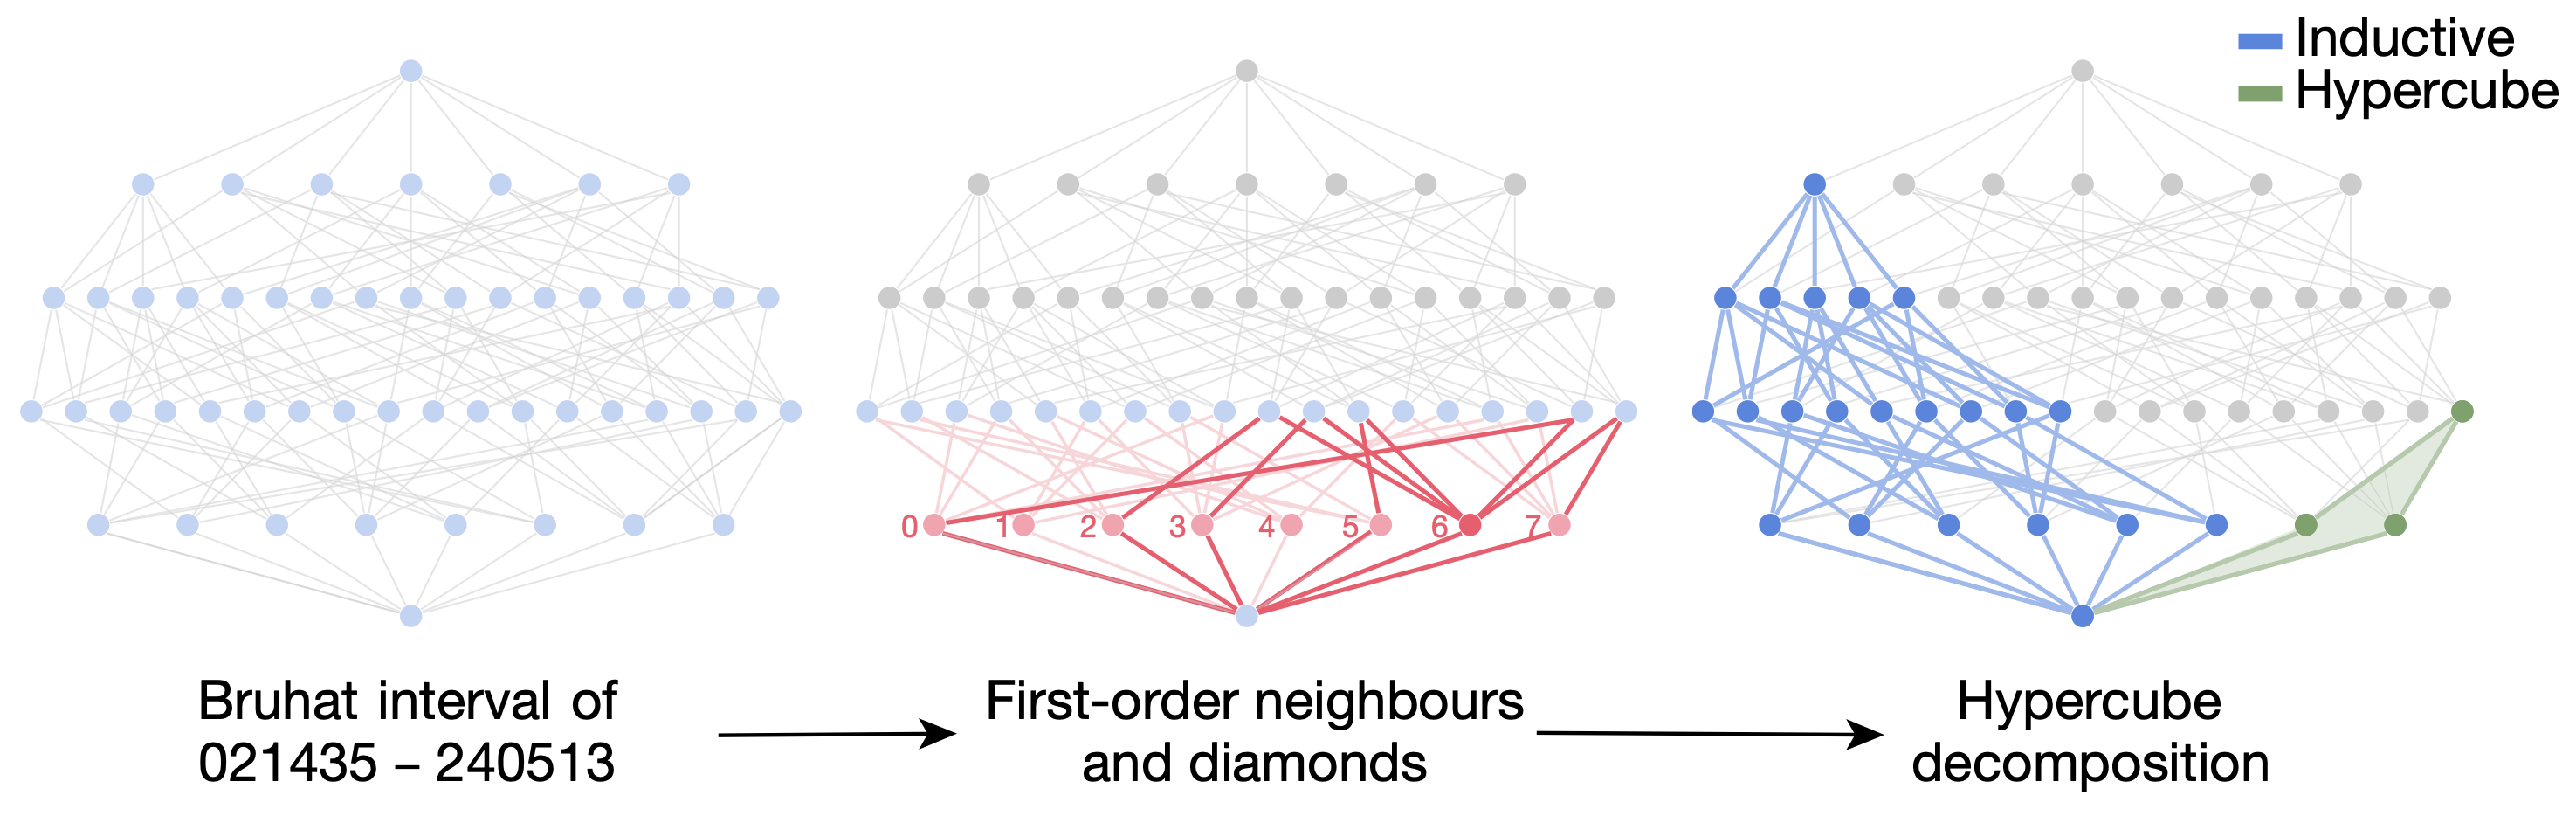
\includegraphics[height=3.2cm]{./figures/hypercube.png}
  \end{center}
  }

  \only<4>{
  \begin{conjecture}[Hypercube decomposition, Blundell et al., 2022]
    For \( u \le v \) in the symmetric group, \( P_{u,v}(q) \) is determined by
    a recursive formula along a hypercube decomposition of \( [u,v] \).
  \end{conjecture}
  }
\end{frame}

%%%%%%%%%%%%%%%%%%%%%%%%%%%%%%%%%%%%%%%%%%%%%%

\begin{frame}
  \frametitle{Case 2: Murmurations of elliptic curves}
  \vspace{-.8cm}
  \begin{columns}[T]
    \begin{column}{.34\textwidth}
      \begin{center}
        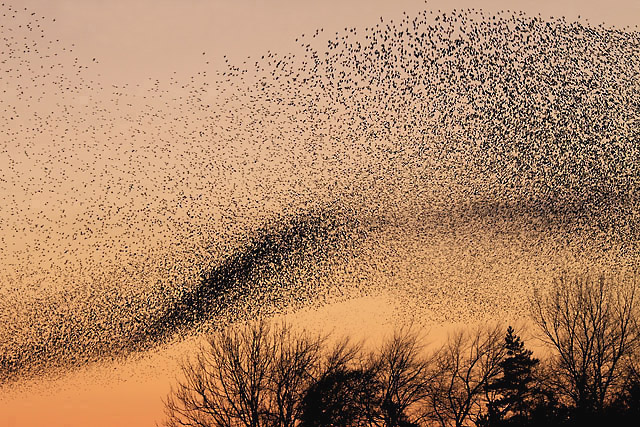
\includegraphics[width=\textwidth]{./figures/Starling_murmuration.jpeg} \\
        {\footnotesize Starling murmuration}
      \end{center}
    \end{column}
    \begin{column}{.43\textwidth}
      \begin{center}
        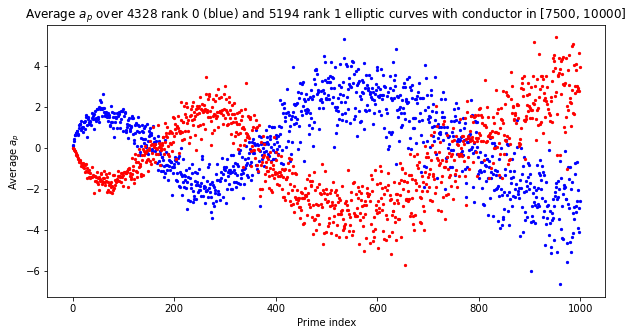
\includegraphics[width=\textwidth]{./figures/murmuration_apPlot.png} \\
        {\footnotesize Averaged \( a_p \) for elliptic curves, \( N \in [7500,10000] \)}
      \end{center}
    \end{column}
  \end{columns}
  \pause

  \begin{conjecture}[He--Lee--Oliver--Pozdnyakov, 2022]
    There exist continuous functions \( M_r : \RR_{>0} \to \RR \) such that,
    for \( r \in \{0,1\} \),
    \[
      \frac{1}{\#\mathcal{E}_r(N)} \sum_{\substack{E \in \mathcal{E}_r(N) \\ p \approx yN}} a_p(E)
      \;\longrightarrow\; M_r(y) \qquad (N \to \infty),
    \]
    where \( \mathcal{E}_r(N) \) is the set of curves of rank \( r \) with
    \( N_E \in [N, 2N] \).
  \end{conjecture}
\end{frame}

%%%%%%%%%%%%%%%%%%%%%%%%%%%%%%%%%%%%%%%%%%%%%%

\begin{frame}
  \frametitle{Reformulating problems for AI}
  \pause
  In both cases, the decisive step was not the machine learning itself,
  but reformulating the problem into a form that a learning model can work
  with. \vspace{.3cm}
  \pause

  Typically this requires
  \begin{itemize}
    \item[$\bullet$] a large family of examples,
    \item[$\bullet$] a concrete numerical or computable target, and
    \item[$\bullet$] a representation of the input that preserves the
      relevant structure.
  \end{itemize}
  % \vspace{.3cm}
  % \pause

  % I will now describe two problems from my own research where I am trying
  % to carry out such a reformulation.
\end{frame}

%%%%%%%%%%%%%%%%%%%%%%%%%%%%%%%%%%%%%%%%%%%%%%

\begin{frame}
  \frametitle{A: The \( e \)-positivity conjecture}
  For a Hessenberg function \( h \), write the chromatic symmetric function as
  \[
    X_h(\xx) = \sum_{\lambda} c_\lambda\, e_\lambda(\xx).
  \]
  \pause
  \begin{StanleyStembridge}
    For every Hessenberg function \( h \), \( c_\lambda \ge 0 \).
  \end{StanleyStembridge}
  \pause

  \begin{thm}[Gasharov, 1996; Shareshian--Wachs, 2016; Hwang, 2024]
    \[
      c_\lambda \;\le\; \#\{P\text{-tableaux of shape } \lambda\}.
    \]
  \end{thm}
\end{frame}

%%%%%%%%%%%%%%%%%%%%%%%%%%%%%%%%%%%%%%%%%%%%%%

\begin{frame}
  \frametitle{A: The \( e \)-positivity conjecture}
  \textbf{Example.} Let \( h = (2,4,5,5,6,6) \). Then the \( P \)-tableaux of
  shape \( (4,2) \) are:
  \vspace{.2cm}
  \begin{center}
    \begin{tabular}{ccc}
      {\begin{ytableau} 2 & 1 & 3 & 4 \\ 5 & 6 \end{ytableau}} &
      {\begin{ytableau} 2 & 1 & 4 & 6 \\ 5 & 3 \end{ytableau}} &
      {\color<5->{red}\begin{ytableau} 1 & 2 & 5 & 4 \\ 3 & 6 \end{ytableau}} \\[2em]
      {\color<5->{red}\begin{ytableau} 1 & 3 & 2 & 4 \\ 5 & 6 \end{ytableau}} &
      {\color<5->{red}\begin{ytableau} 1 & 2 & 3 & 4 \\ 6 & 5 \end{ytableau}} &
      {\begin{ytableau} 1 & 4 & 2 & 5 \\ 3 & 6 \end{ytableau}}
    \end{tabular}
  \end{center}
  \vspace{.2cm}

  \onslide<3->{
  \textbf{Reformulation.} \emph{Find a `good' condition on \( P \)-tableaux
  such that the \( e \)-coefficient \( c_\lambda \) counts good \( P \)-tableaux
  of shape \( \lambda \).}
  \vspace{.15cm}
  }

  \onslide<4->{
  We approach this using a graph neural network.
  }

  \onslide<6->{
  \begin{conjecture}[Hwang--Min, 2026+]
    \[
      c_\lambda \;\le\; \#\{\text{backward-connected } P\text{-tableaux of shape } \lambda\}.
    \]
  \end{conjecture}
  }
\end{frame}

%%%%%%%%%%%%%%%%%%%%%%%%%%%%%%%%%%%%%%%%%%%%%%

\begin{frame}
  \frametitle{B: Schubert structure constants}
  For each permutation \( w \in S_n \), the \emph{Schubert polynomial}
  \( \mathfrak{S}_w \in \ZZ[x_1,x_2,\ldots] \) represents the class of the
  Schubert variety \( X_w \) in the cohomology of the flag variety
  \( \mathrm{Fl}_n \). Their products define the \remph{Schubert structure
  constants} \( c^w_{u,v} \in \ZZ \):
  \[
    \mathfrak{S}_u \cdot \mathfrak{S}_v \;=\; \sum_w c^w_{u,v}\, \mathfrak{S}_w,
    \qquad
    [X_u] \cdot [X_v] \;=\; \sum_w c^w_{u,v}\, [X_w] \;\text{ in } H^*(\mathrm{Fl}_n).
  \]
  \pause
  Geometrically \( c^w_{u,v} \ge 0 \), by transversal intersection.
  \pause

  \begin{OpenProblem}
    For permutations \( w, u, v \), find an algebraic/combinatorial proof
    that \( c^w_{u,v} \ge 0 \).
  \end{OpenProblem}
\end{frame}

%%%%%%%%%%%%%%%%%%%%%%%%%%%%%%%%%%%%%%%%%%%%%%

\begin{frame}
  \frametitle{B: The Fomin--Kirillov algebra}
  \begin{defn}[Fomin--Kirillov, 1999]
    \( \mathcal{E}_n \) is the algebra generated by \( \{x_{ij} : 1 \le i < j \le n\} \)
    subject to
    \begin{itemize}
      \item[$\bullet$] \( x_{ij}^2 = 0 \);
      \item[$\bullet$] \( x_{ij}x_{kl} = x_{kl}x_{ij} \) if \( \{i,j\} \cap \{k,l\} = \emptyset \);
      \item[$\bullet$] \( x_{ij}x_{jk} + x_{jk}x_{ki} + x_{ki}x_{ij} = 0 \) for distinct \( i,j,k \).
    \end{itemize}
  \end{defn}
  \pause

  For \( 1 \le i \le n \), the \emph{Dunkl element} is
  \(
    \theta_i = \sum_{j \ne i} x_{ij} \in \mathcal{E}_n.
  \)
  % The \( \theta_i \)'s pairwise commute, and
  % \(
  %   \QQ[\theta_1,\ldots,\theta_{n-1}] \cong H^*(\mathrm{Fl}_n;\QQ).
  % \)
  % In particular, each Schubert polynomial \( \mathfrak{S}_w \) can be
  % evaluated at the Dunkl elements, yielding \( \mathfrak{S}_w(\theta) \in \mathcal{E}_n \).
  \pause
  \vspace{.15cm}

  Let \( \mathcal{E}_n^+ \subset \mathcal{E}_n \) be the \emph{positive cone}: the
  \( \QQ_{\ge 0} \)-span of monomials in the generators \( x_{ij} \) (\( i<j \)).
  \pause

  \begin{FKnonneg}
    For every \( w \in S_n \),
    \(
      \mathfrak{S}_w(\theta_1, \ldots, \theta_{n-1}) \in \mathcal{E}_n^+.
    \)
  \end{FKnonneg}
  % \pause

  % \vspace{.1cm}
  % Since \( \mathcal{E}_n^+ \) is closed under multiplication, this would
  % immediately imply \( c^w_{u,v} \ge 0 \) algebraically---and yield an
  % \emph{explicit} monomial expression for each \( c^w_{u,v} \).
\end{frame}

%%%%%%%%%%%%%%%%%%%%%%%%%%%%%%%%%%%%%%%%%%%%%%

\begin{frame}[fragile]
  \frametitle{B: The Fomin--Kirillov algebra}
  For \( w = 3214 \in S_4 \), expanding \( \mathfrak{S}_w(\theta) \) and
  repeatedly applying the FK relations:
  \only<1>{\begin{align*}
    \mathfrak{S}_w(\theta) \;=\;
      &\phantom{{}+{}}
        x_{12}x_{13}x_{23} + x_{12}x_{13}x_{24} + x_{12}x_{14}x_{23} + x_{12}x_{14}x_{24} + x_{13}x_{12}x_{23} \\
      &+ \underline{x_{13}x_{12}x_{24}} + x_{13}x_{14}x_{23} + x_{13}x_{14}x_{24} + x_{14}x_{12}x_{23} + x_{14}x_{12}x_{24} \\
      &+ x_{14}x_{13}x_{23} + x_{14}x_{13}x_{24} - x_{12}x_{13}x_{12} - x_{12}x_{14}x_{12} - x_{13}x_{14}x_{12} \\
      &- x_{14}x_{13}x_{12}.
  \end{align*}
  \vspace{-.6cm}
  \[
    x_{13}x_{12}x_{24} \;\Rightarrow\; x_{13}x_{14}x_{12} \;+\; x_{13}x_{24}x_{14}.
  \]}
  \only<2>{\begin{align*}
    \mathfrak{S}_w(\theta) \;=\;
      &\phantom{{}+{}}
        x_{12}x_{13}x_{23} + x_{12}x_{13}x_{24} + x_{12}x_{14}x_{23} + x_{12}x_{14}x_{24} + x_{13}x_{12}x_{23} \\
      &+ x_{13}x_{14}x_{23} + x_{13}x_{14}x_{24} + x_{13}x_{24}x_{14} + \underline{x_{14}x_{12}x_{23}} + x_{14}x_{12}x_{24} \\
      &+ x_{14}x_{13}x_{23} + x_{14}x_{13}x_{24} - x_{12}x_{13}x_{12} - x_{12}x_{14}x_{12} - x_{14}x_{13}x_{12}.
  \end{align*}
  \vspace{-.6cm}
  \[
    x_{14}x_{12}x_{23} \;\Rightarrow\; x_{14}x_{13}x_{12} \;+\; x_{14}x_{23}x_{13}.
  \]}
  \only<3>{\begin{align*}
    \mathfrak{S}_w(\theta) \;=\;
      &\phantom{{}+{}}
        x_{12}x_{13}x_{23} + x_{12}x_{13}x_{24} + x_{12}x_{14}x_{23} + x_{12}x_{14}x_{24} + x_{13}x_{12}x_{23} \\
      &+ x_{13}x_{14}x_{23} + x_{13}x_{14}x_{24} + x_{13}x_{24}x_{14} + x_{14}x_{12}x_{24} + x_{14}x_{13}x_{23} \\
      &+ x_{14}x_{13}x_{24} + x_{14}x_{23}x_{13} \underline{{}- x_{12}x_{13}x_{12}} - x_{12}x_{14}x_{12}.
  \end{align*}
  \vspace{-.6cm}
  \[
    -\,x_{12}x_{13}x_{12} \;\Rightarrow\; -\,x_{23}x_{12}x_{12} \;+\; x_{13}x_{23}x_{12}.
  \]}
  \only<4>{\begin{align*}
    \mathfrak{S}_w(\theta) \;=\;
      &\phantom{{}+{}}
        x_{12}x_{13}x_{23} + x_{12}x_{13}x_{24} + x_{12}x_{14}x_{23} + x_{12}x_{14}x_{24} + x_{13}x_{12}x_{23} \\
      &+ x_{13}x_{14}x_{23} + x_{13}x_{14}x_{24} + x_{13}x_{23}x_{12} + x_{13}x_{24}x_{14} + x_{14}x_{12}x_{24} \\
      &+ x_{14}x_{13}x_{23} + x_{14}x_{13}x_{24} + x_{14}x_{23}x_{13} \underline{{}- x_{12}x_{14}x_{12}}.
  \end{align*}
  \vspace{-.6cm}
  \[
    -\,x_{12}x_{14}x_{12} \;\Rightarrow\; -\,x_{24}x_{12}x_{12} \;+\; x_{14}x_{24}x_{12}.
  \]}
  \only<5->{\begin{align*}
    \mathfrak{S}_w(\theta) \;=\;
      &\phantom{{}+{}}
        x_{12}x_{13}x_{23} + x_{12}x_{13}x_{24} + x_{12}x_{14}x_{23} + x_{12}x_{14}x_{24} + x_{13}x_{12}x_{23} \\
      &+ x_{13}x_{14}x_{23} + x_{13}x_{14}x_{24} + x_{13}x_{23}x_{12} + x_{13}x_{24}x_{14} + x_{14}x_{12}x_{24} \\
      &+ x_{14}x_{13}x_{23} + x_{14}x_{13}x_{24} + x_{14}x_{23}x_{13} + x_{14}x_{24}x_{12}.
  \end{align*}}
  \normalsize
  \onslide<6->{
  \textbf{Reformulation.} \emph{Starting from the initial state
  \( \mathfrak{S}_w(\theta) \), find a path---via FK rewrites---into the
  positive cone \( \mathcal{E}_n^+ \).} \vspace{.15cm}

  \textbf{Approach.} I am attacking this search problem with
  \remph{reinforcement learning}.}
\end{frame}

%%%%%%%%%%%%%%%%%%%%%%%%%%%%%%%%%%%%%%%%%%%%%%

\section{Interactive \& automated theorem proving}

%%%%%%%%%%%%%%%%%%%%%%%%%%%%%%%%%%%%%%%%%%%%%%

\begin{frame}
  \frametitle{Two flavors of AI-assisted proving}
  \pause
  \begin{center}
    \renewcommand{\arraystretch}{1.3}
    \footnotesize
    \resizebox{\textwidth}{!}{%
    \begin{tabular}{|c|c|c|}
      \hline
        & \textbf{Construction} & \textbf{Automated proving} \\
      \hline\hline
      Goal & Find an object / counterexample & Produce a formal proof \\
      \hline
      Output & An explicit witness & A machine-checked proof term \\
      \hline
      Examples & AlphaEvolve, PatternBoost & AlphaProof, Aristotle \\
      \hline
      Core tool & Search + LLM / evolution & Proof assistants (Lean, \ldots) \\
      \hline
    \end{tabular}}
  \end{center}
  \pause
  \vspace{.3cm}

  The two directions are complementary: construction narrows down a
  conjecture to a concrete statement, while automated proving certifies
  it once the statement is in place.
\end{frame}

%%%%%%%%%%%%%%%%%%%%%%%%%%%%%%%%%%%%%%%%%%%%%%

\begin{frame}
  \frametitle{Math research agents}
  Beyond single tools, \remph{autonomous research agents} are now being
  built on top of LLMs, proof assistants, and search: they formulate
  subgoals, call solvers, verify proofs, and iterate---with very little
  human interaction.
\end{frame}

%%%%%%%%%%%%%%%%%%%%%%%%%%%%%%%%%%%%%%%%%%%%%%

\begin{frame}
  \frametitle{Math research agents}
  \begin{center}
    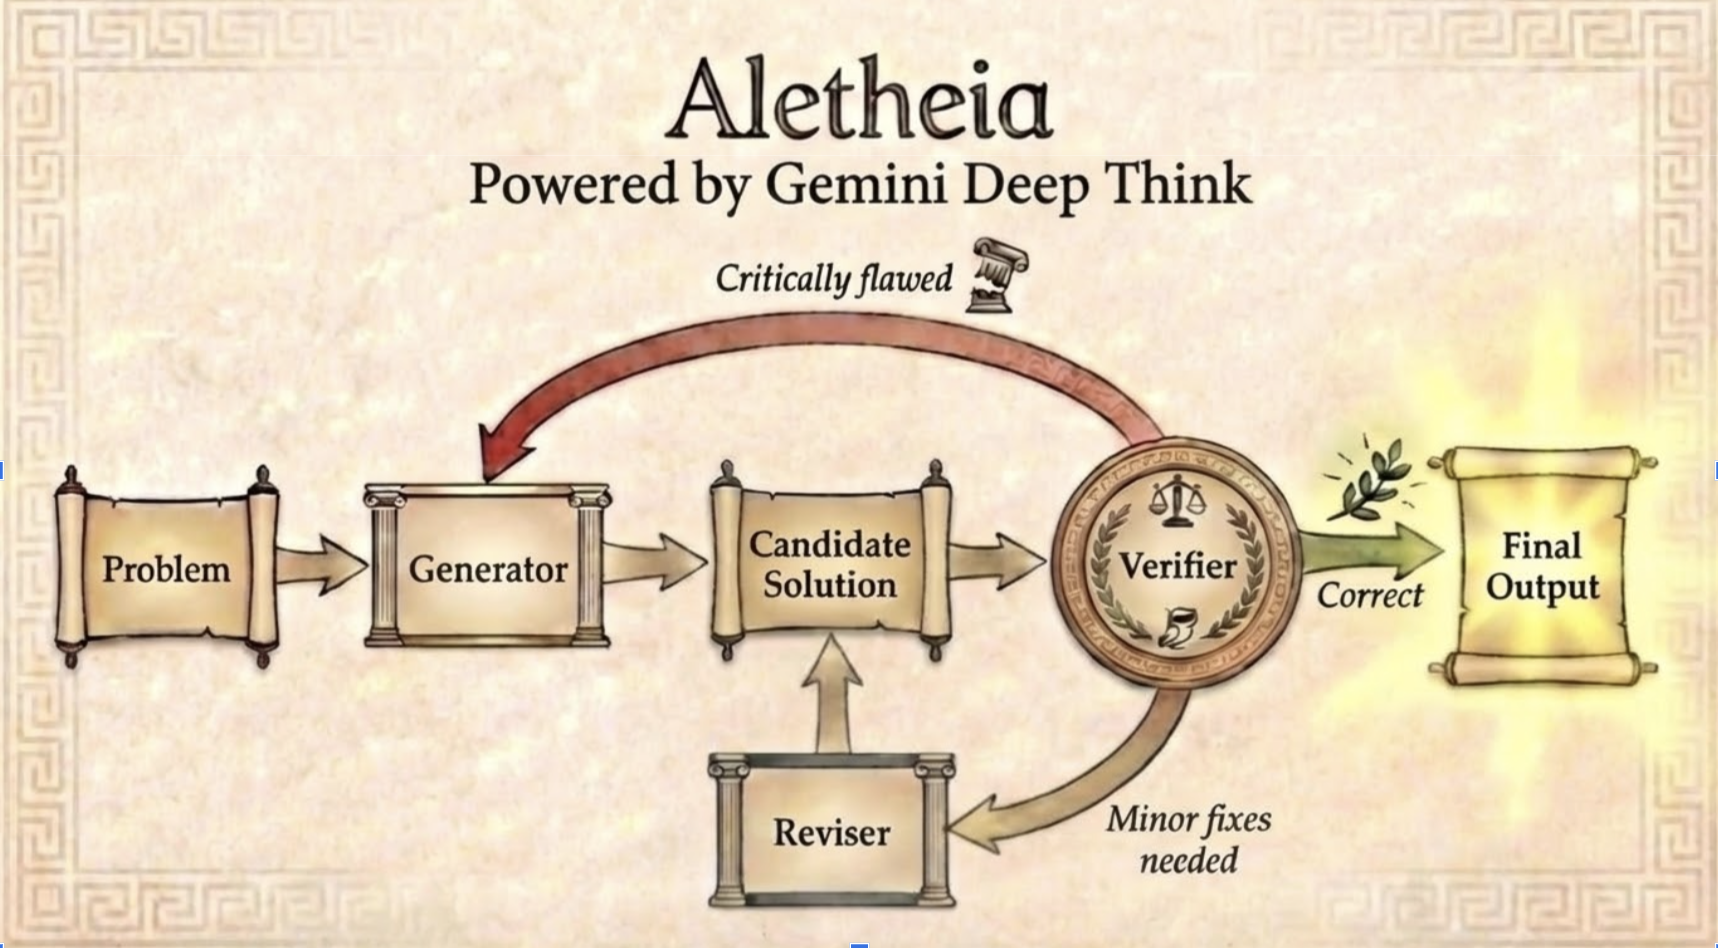
\includegraphics[width=\textwidth]{./figures/Aletheia.png} \\
    \vspace{.2cm}
    {\small Aletheia (Google DeepMind)}
  \end{center}
\end{frame}

%%%%%%%%%%%%%%%%%%%%%%%%%%%%%%%%%%%%%%%%%%%%%%

\begin{frame}
  \frametitle{Math research agents}
  \begin{center}
    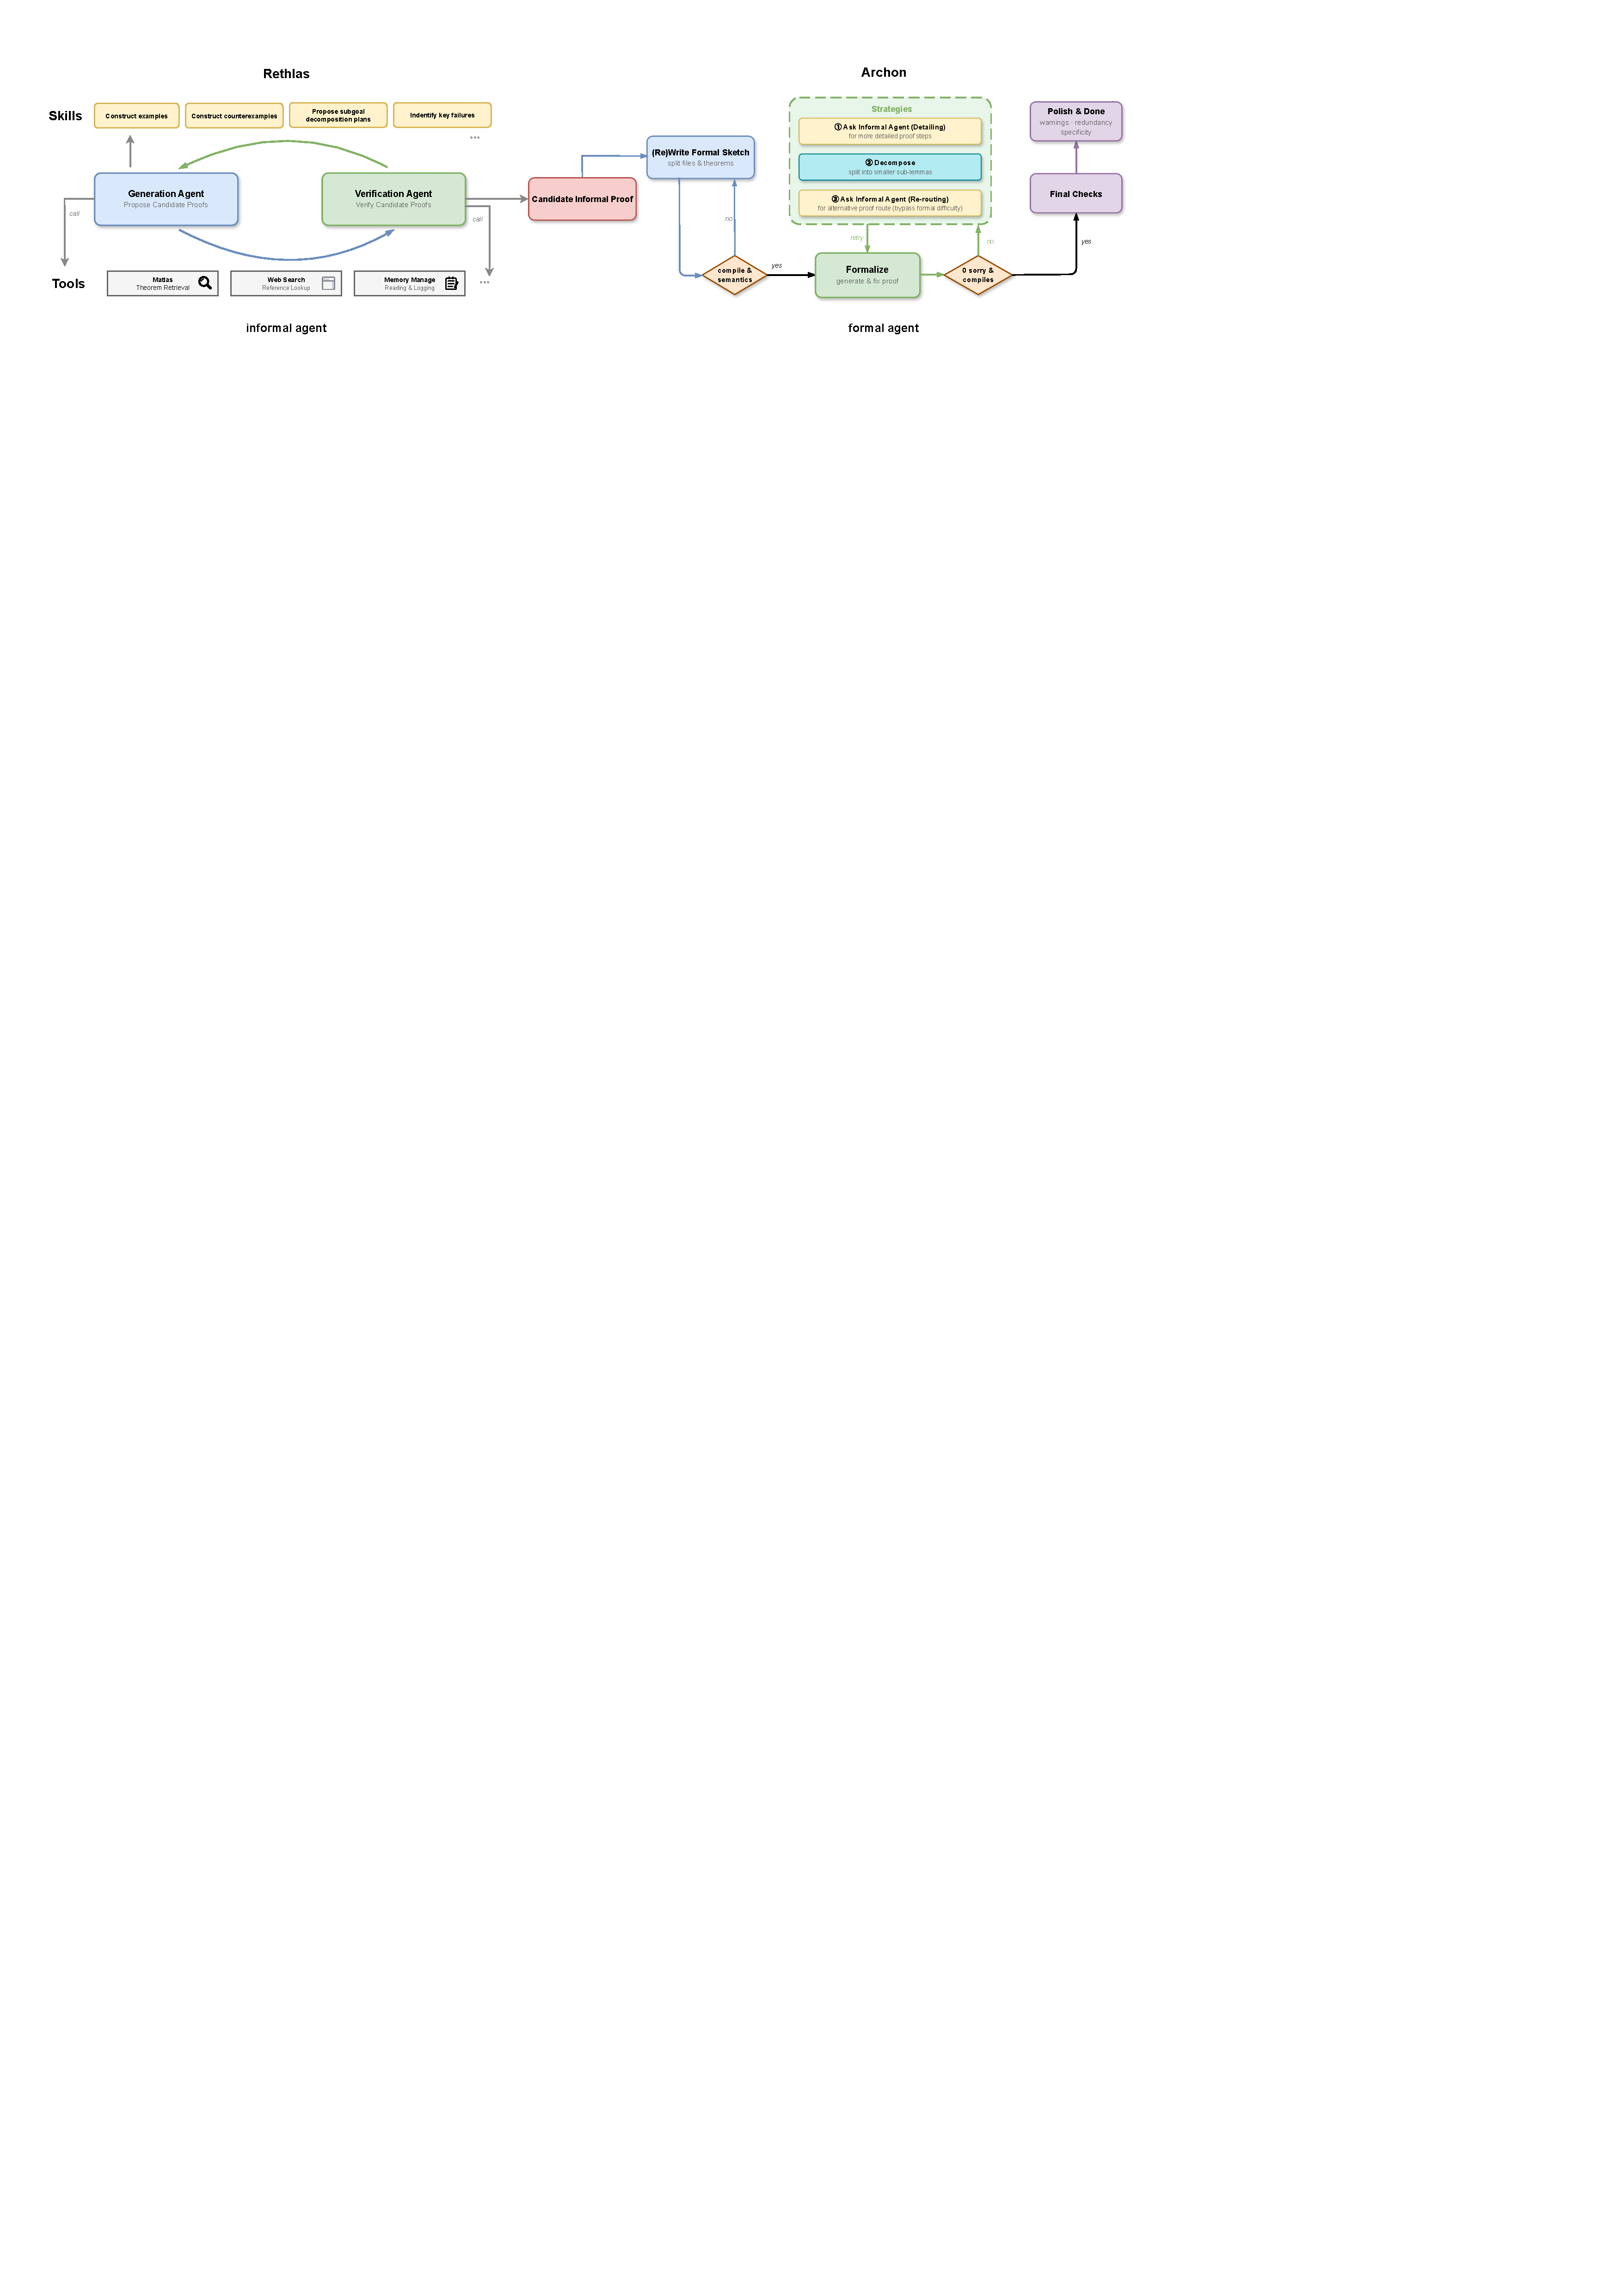
\includegraphics[width=\textwidth]{./figures/rethlas-archon.pdf} \\
    \vspace{.2cm}
    {\small Rethlas--Archon (Bin Dong et al.)}
  \end{center}
\end{frame}

%%%%%%%%%%%%%%%%%%%%%%%%%%%%%%%%%%%%%%%%%%%%%%

\begin{frame}
  \frametitle{Math research agents}
  Currently I am building a research-agent pipeline aimed at a concrete
  open problem. Two specialized sub-agents cooperate: a
  \bemph{mathematical-reasoning agent} (proposes ideas, writes proofs)
  and a \bemph{code-execution agent} (runs exact-computational checks and
  verifies proof steps).
  \vspace{.2cm}

  \begin{center}
  \begin{tikzpicture}[
    >={Latex[length=2mm]},
    node distance=0.4cm and 0.35cm,
    every node/.append style={font=\scriptsize},
    box/.style={rectangle, rounded corners=2pt, draw, semithick,
                minimum height=0.8cm, minimum width=1.9cm, align=center,
                fill=white},
    mbox/.style={box, fill=blue!12},
    cbox/.style={box, fill=orange!18},
    dec/.style={diamond, draw, semithick, aspect=2.2, fill=gray!15,
                inner sep=0pt, align=center, minimum width=1.2cm},
  ]
    \node[box] (S) {Strategy\\ selection};
    \node[mbox, right=of S] (E) {Mathematical\\ exploration};
    \node[cbox, right=of E] (V) {Code\\ verification};
    \node[box, right=of V] (O) {Observation\\ (commit)};
    \node[dec, below=0.55cm of O] (F) {Provable?};
    \node[mbox, left=of F] (P) {Proof\\ writing};
    \node[cbox, left=of P] (PV) {Proof\\ verification};
    \node[box, left=of PV] (D) {$\checkmark$\ Done};

    \draw[->,semithick] (S) -- (E);
    \draw[->,semithick] (E) -- (V);
    \draw[->,semithick] (V) -- (O);
    \draw[->,semithick] (O) -- (F);
    \draw[->,semithick] (F) -- node[above,font=\tiny]{yes} (P);
    \draw[->,semithick] (P) -- (PV);
    \draw[->,semithick] (PV) -- node[above,font=\tiny]{ok} (D);

    \coordinate (LB) at ([xshift=-0.45cm, yshift=-0.75cm]D.south west);
    \draw[->,semithick] (F.south) |- (LB) |- (S.west);
    \draw[semithick] (PV.south) |- (LB);
    \node[font=\tiny, fill=white, inner sep=1pt, below=8pt of F.south, anchor=north] {no};
    \node[font=\tiny, fill=white, inner sep=1pt, below=6pt of PV.south, anchor=north] {fail};
  \end{tikzpicture}
  \end{center}
\end{frame}

%%%%%%%%%%%%%%%%%%%%%%%%%%%%%%%%%%%%%%%%%%%%%%

\begin{frame}
  \frametitle{A new theorem via the pipeline}
  The Temperley--Lieb algebra \( \TL_n(q) \) has two distinguished bases,
  indexed by partitions \( \lambda \subseteq Y_n \):
  \begin{itemize}
    \item[$\bullet$] the \bemph{Kazhdan--Lusztig basis} \( \{ \KL_\lambda \} \),
    \item[$\bullet$] the \bemph{monomial basis} \( \{ E_\lambda \} \).
  \end{itemize}
  \pause
  \vspace{.15cm}

  \textbf{Question.} What are the entries of the transition matrices
  \( (\KL_\lambda \to E_\mu) \) and \( (E_\lambda \to \KL_\mu) \)?
  \pause
  \vspace{.15cm}

  To each pair \( \mu \subseteq \lambda \) we associate the \remph{generalized
  chord diagram} \( c(\mu,\lambda) \): draw \( \mu \) as upper arcs and
  \( \lambda \) as lower arcs on a row of dots. It decomposes into
  \emph{strands} (good / bad) and \emph{loops}:
  \vspace{.1cm}
  \begin{center}
    \begin{tikzpicture}[scale=0.55, every node/.style={font=\scriptsize}]
      \foreach \x in {1,...,7} \draw (\x,0) node[circle, fill=black, inner sep=1pt] {};
      \draw (1,0) ..controls(2,1.4) and (5,1.4).. (6,0);
      \draw (2,0) ..controls(2,.6) and (3,.6).. (3,0);
      \draw (4,0) ..controls(4,.6) and (5,.6).. (5,0);
      \node at (7,.55) {\( \mathsf{R} \)};
      \draw (2,0) ..controls(3,-1.4) and (6,-1.4).. (7,0);
      \draw (3,0) ..controls(3.4,-1.0) and (5.6,-1.0).. (6,0);
      \draw (4,0) ..controls(4,-.6) and (5,-.6).. (5,0);
      \node at (1,-.55) {\( \mathsf{R} \)};
    \end{tikzpicture}
  \end{center}
\end{frame}

%%%%%%%%%%%%%%%%%%%%%%%%%%%%%%%%%%%%%%%%%%%%%%

\begin{frame}
  \frametitle{Result via the pipeline}
  Discovered and verified through our agent pipeline:
  \pause
  Write the expansion as
  \[
    E_\lambda \;=\; \sum_{\mu \subseteq \lambda} G_{\lambda,\mu}\, \KL_\mu.
  \]

  \begin{thm}[H.--Shigechi, 2026+]
    For \( \mu \subseteq \lambda \),
    \[
      G_{\lambda,\mu} \;=\;
      \begin{cases}
        \tau^{\,d(\mu,\lambda)} & \text{if } c(\mu,\lambda) \text{ has no bad strands}, \\[.3em]
        0 & \text{otherwise},
      \end{cases}
    \]
    where \( d(\mu,\lambda) \) is the number of loops in \( c(\mu,\lambda) \)
    and \( \tau = -(q+q^{-1}) \).
  \end{thm}
  \pause

  % A parallel formula describes \( \KL_\lambda \) in the \( E \)-basis via
  % Dyck tilings of mixed type. \vspace{.15cm}

  The combinatorial argument underlying the proof
  % ---matching compatible
  % intermediate paths to arcs in \( c(\mu,\lambda) \)---
  was first spotted by
  the mathematical-reasoning agent and then verified, refined, and proved
  through the loop.
\end{frame}

%%%%%%%%%%%%%%%%%%%%%%%%%%%%%%%%%%%%%%%%%%%%%%

\begin{frame}
  \frametitle{Next-generation agents}
  \only<1>{
  \begin{center}
    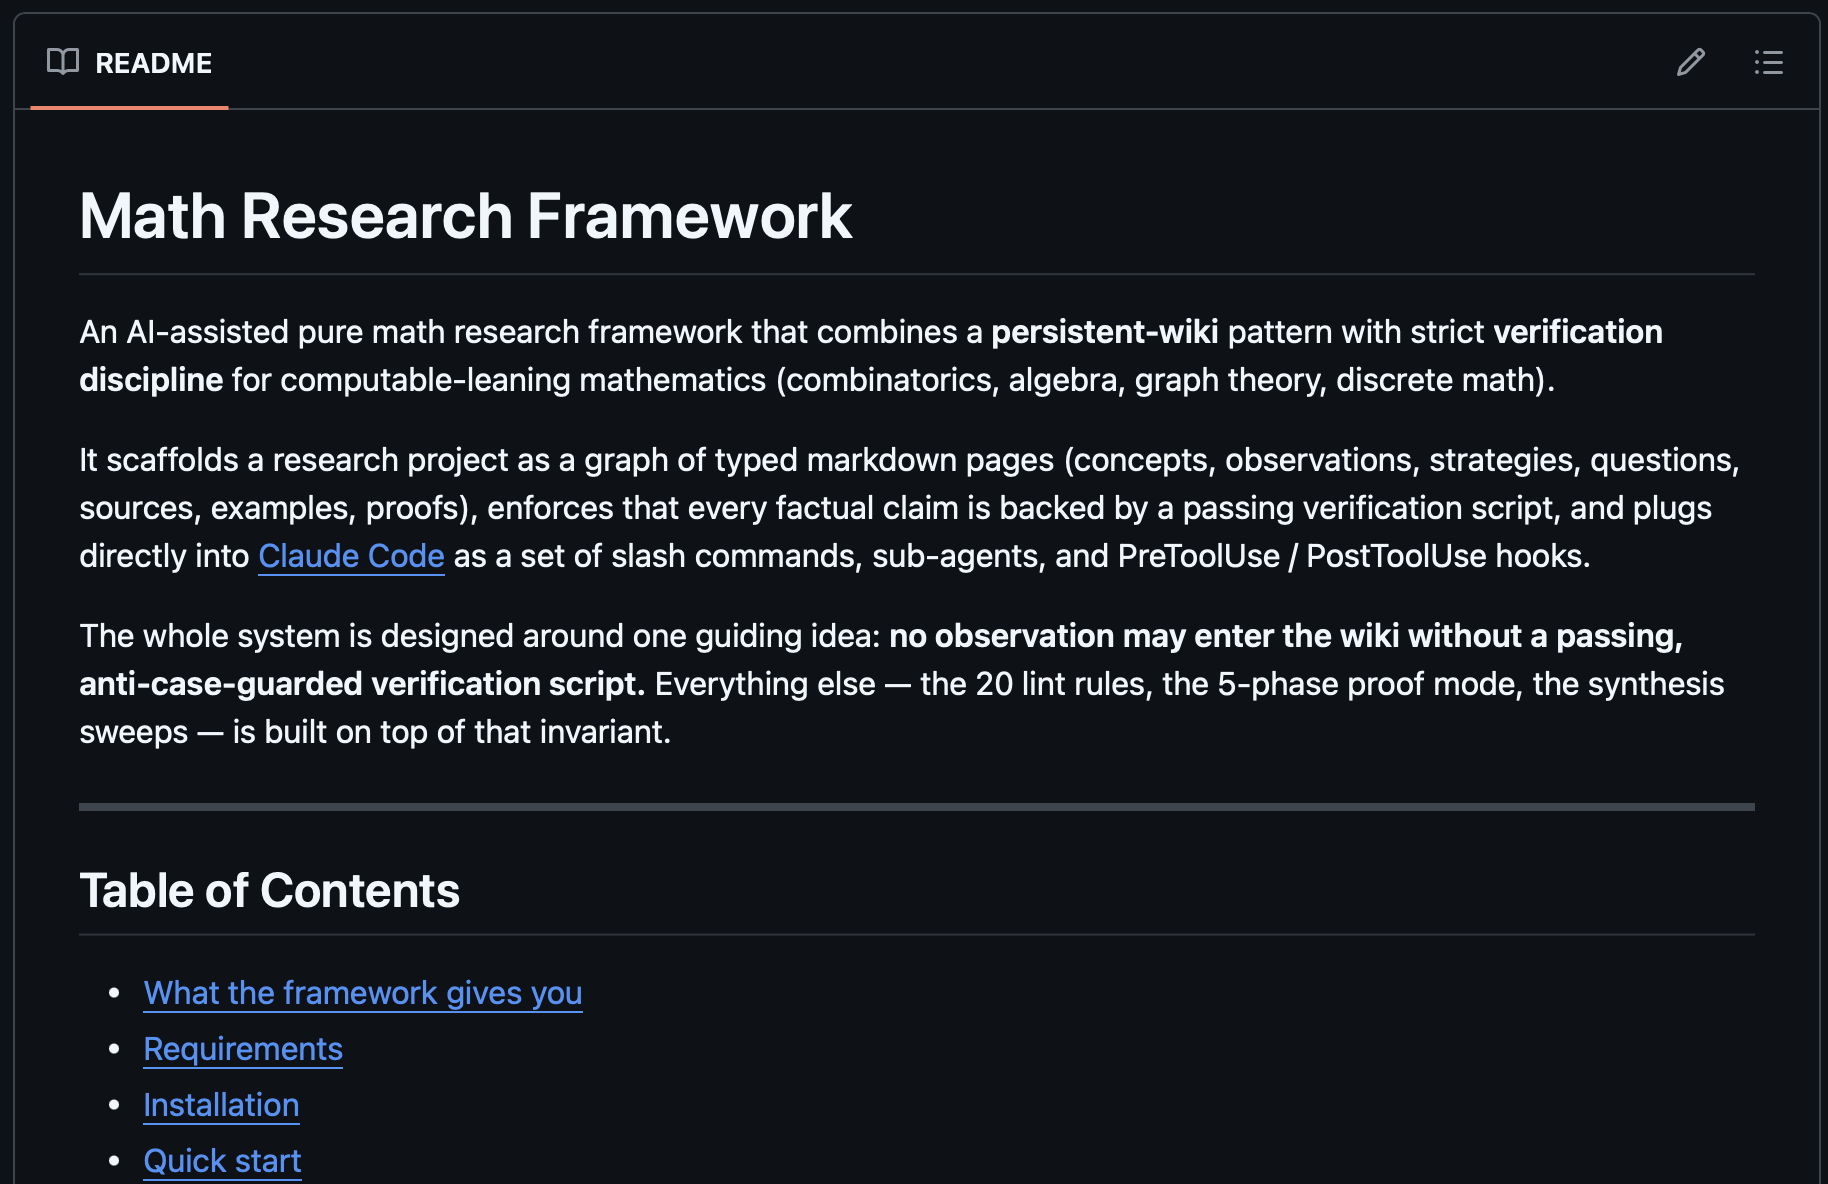
\includegraphics[width=\textwidth]{./figures/new_agent_README.png}
  \end{center}}
  \only<2->{
  \begin{center}
    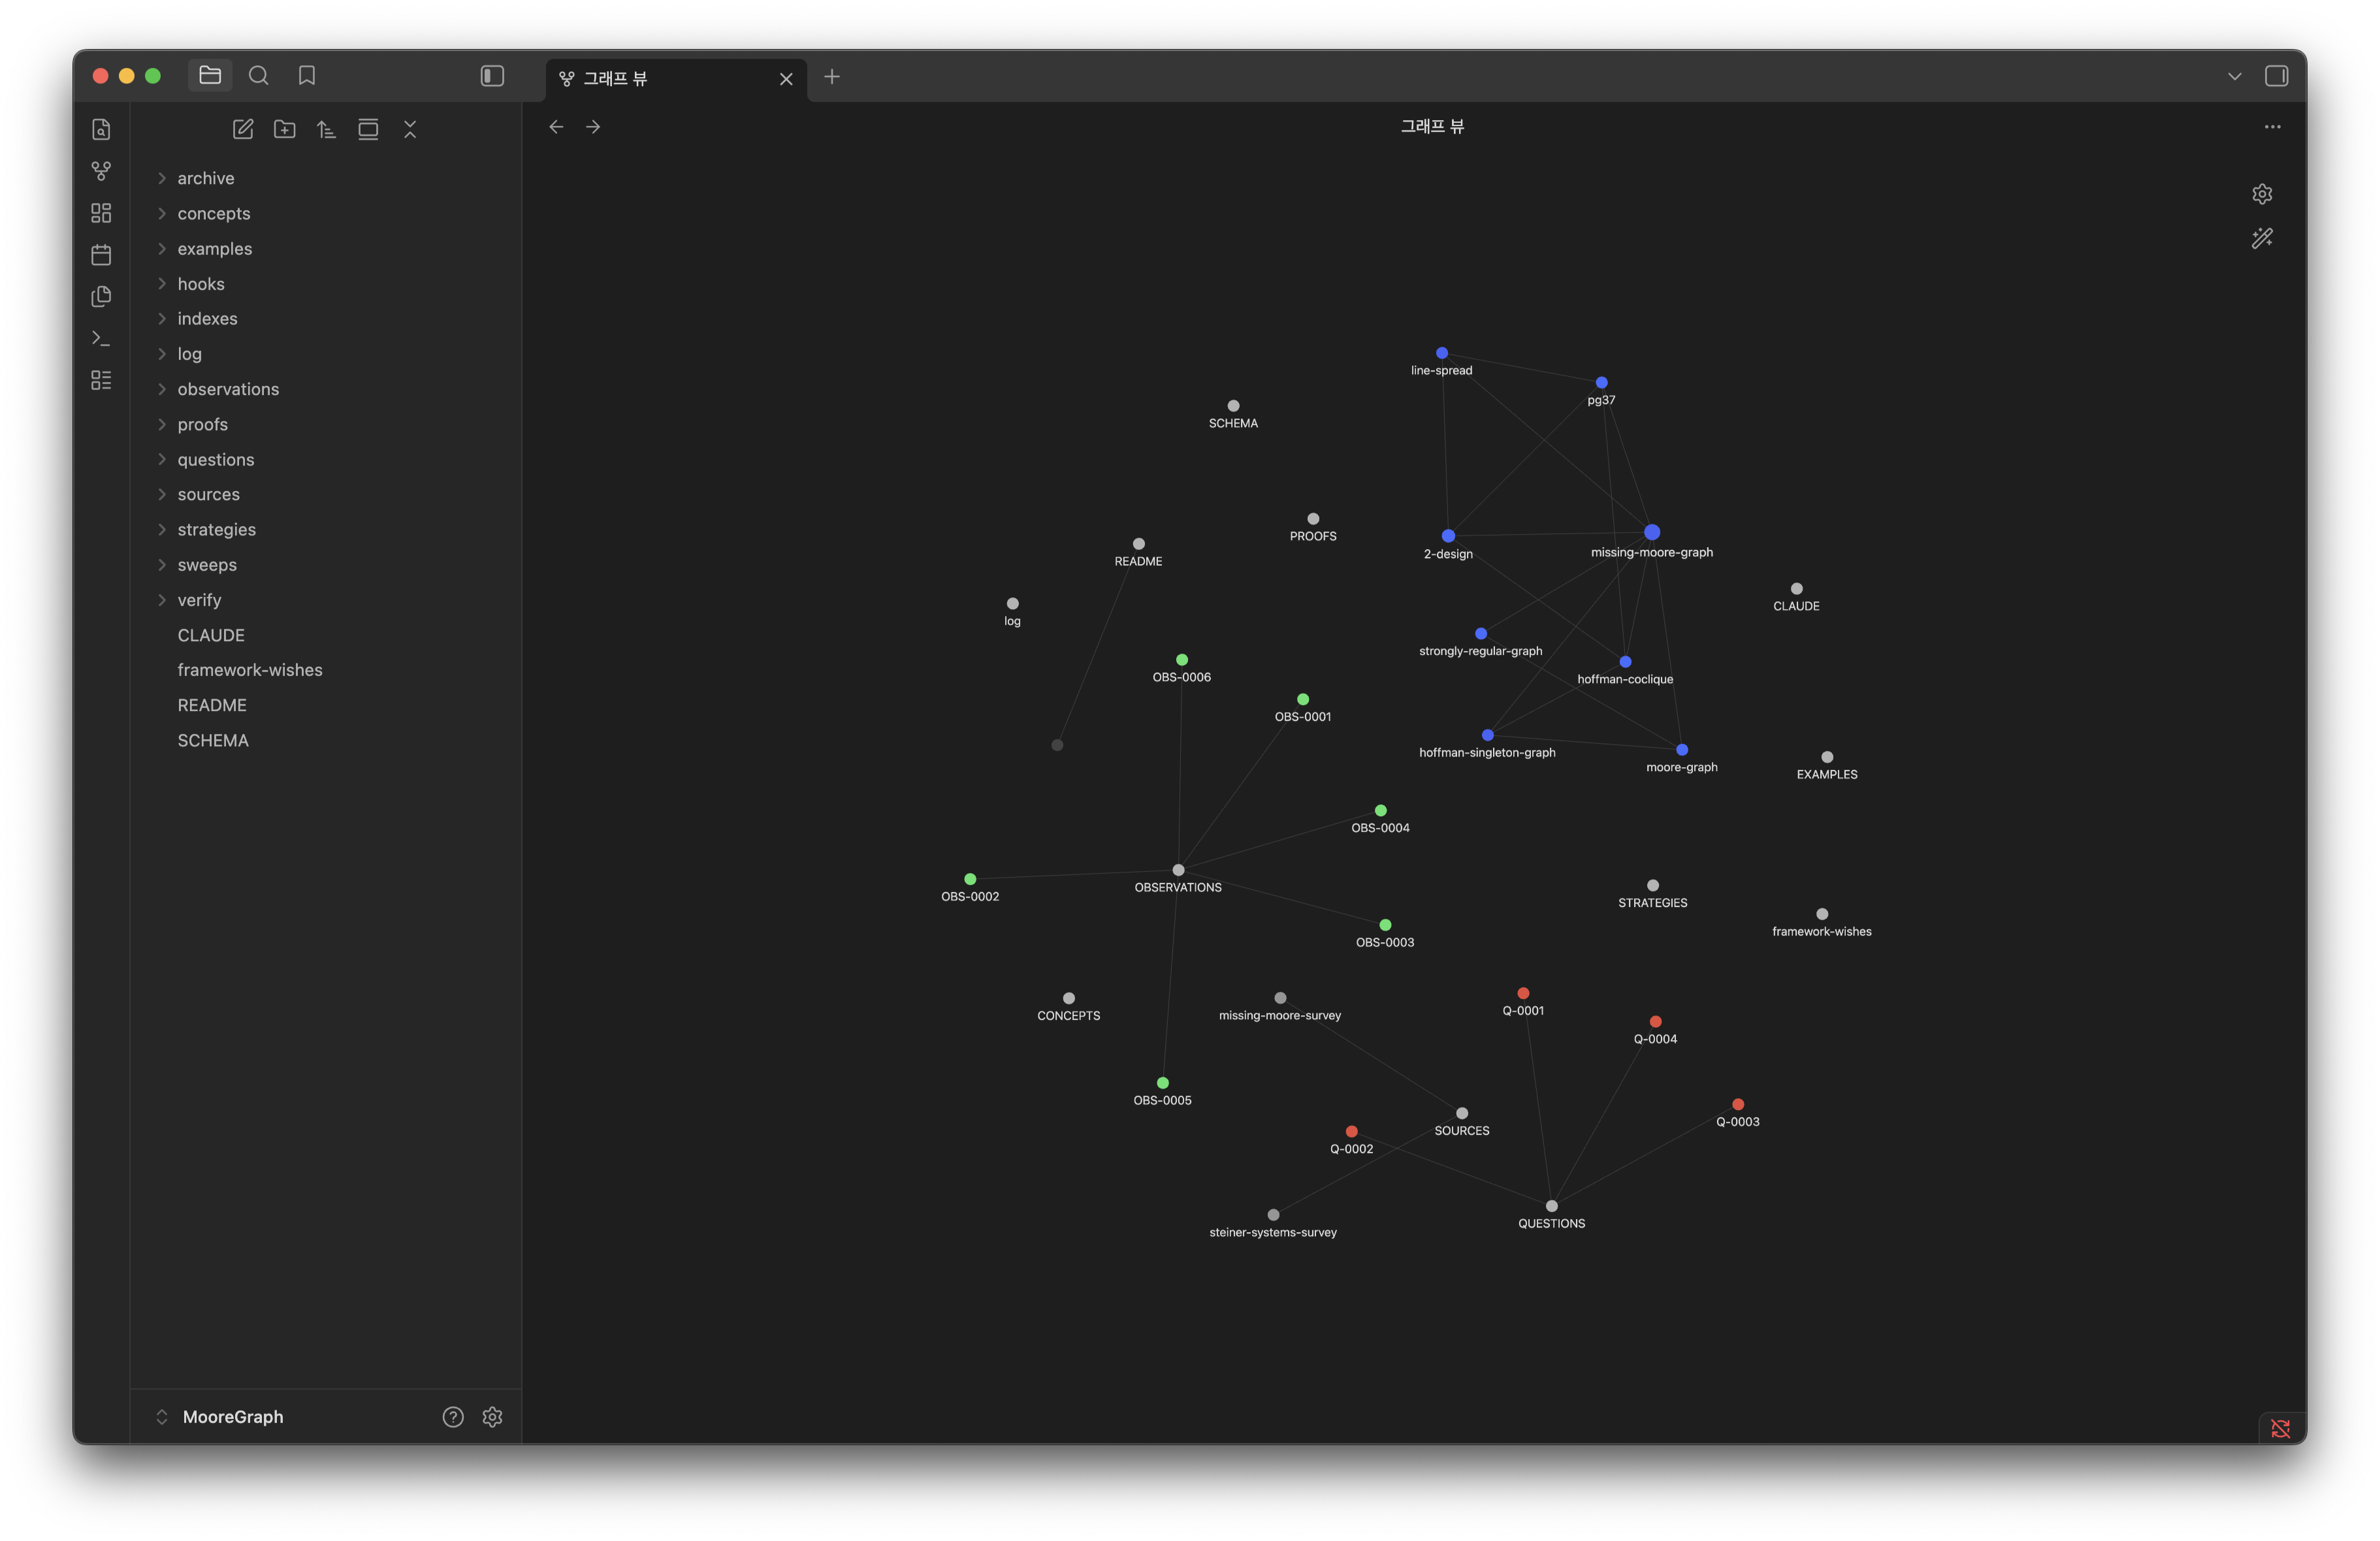
\includegraphics[width=\textwidth]{./figures/new_agent_obsidian.png}
  \end{center}}
\end{frame}

%%%%%%%%%%%%%%%%%%%%%%%%%%%%%%%%%%%%%%%%%%%%%%

\section*{}
\begin{frame}
  \begin{center}
    \Huge Thank you!
  \end{center}
\end{frame}

\end{document}
